

\section{Problem 2}
\label{part2}
\begin{verbatim}

Download the TimeMaps for each of the target URIs.  We'll use the ODU 
Memento Aggregator, so for example:

URI-R = http://www.cs.odu.edu/

URI-T = http://mementoproxy.cs.odu.edu/aggr/timemap/link/1/http://www.cs.odu.edu/

Create a histogram* of URIs vs. number of Mementos (as computed from
the TimeMaps).  For example, 100 URIs with 0 Mementos, 300 URIs
with 1 Memento, 400 URIs with 2 Mementos, etc.

* = https://en.wikipedia.org/wiki/Histogram

\end{verbatim}

\subsection{Solution}
\begin{enumerate}
\item First i played with the memento aggregator in the command prompt and i was getting timemaps for each url and i found mementos in each time map.
\item Now i got to know what to do so i started to write a python code to calculate mementos with urls given as input. 
\item I got a lot of errors and had a hard time working with those. So,I was searching for any other way to find the mementos.
\item I took the URI-T and pasted it in the browser and ran it.Surprisingly a file downloaded and i opened it in notepad++ and 		was happy to see all the time maps in it.
\item So now i switched to this method and used urllib library to run all the urls in the browser and got their respective time maps.
\item I got 404 error for some URI's which indicated that they have no mementos.I had written one function called getmementos(url) in my code to get urls having mementos.
\item Now my next task was to find and count the number of mementos. I used regular expression which finds all the expressions like rel=mementos,rel=first memento and rel=memento last from the time maps..
\item I ran a for loop and counted the number of mementos for each url and saved the url and number of mementos in json format.
\item I observed that out of 1000 only 177 urls had 1 or more mementos and remaining 823 urls had 0 mementos.
\item I wrote code to get 3 output files,one with urls and number of mementos,one csv file only with the number of mementos which is used to give input to R and one json file with urls and number of mementos where number of mementos is greater than zero.  
\item The last file is used to give input to the third question because we need to calculate age for only those urls which have mementos greater than or equal to one.
  
\end{enumerate}
\newpage
\subsection{Code Listing}

\subsubsection{Code for counting mementos for each url}
\lstinputlisting[language=Python,breaklines = true,frame=single,caption={Python program for counting mementos}, label=lst:q1-1,captionpos=b,numbers=left,showspaces=false,showstringspaces=false,basicstyle=\footnotesize]{get_memento_count.py}
\newpage
\subsubsection{R code for histogram}
\lstinputlisting[language=R,breaklines = true,frame=single,caption={R program for generating the histograms for Question 2}, label=lst:q2R,captionpos=b,numbers=left,showspaces=false,showstringspaces=false,basicstyle=\footnotesize]{R_code_hist.R}
\begin{enumerate}
\item I had gone through the R tutorial once before plotting histogram with this data.
\item Then i passed my mementos count to R. Code used for R is shown above.
\item Histogram takes only one input and the frequency of the input is automatically taken on y-axis. 
\item My first histogram graph is shown below. This graph shows that more than 800 urls have 0 mementos and very small number of urls have 1 or more mementos.
\item I wanted to elaborate this graph to show the number of urls that have greater than or equal to 1 memento. So, I scaled the histogram.
\item X-axis is scaled from 0 to 150 using xlim and y-axis is scaled from 0 to 200 using ylim. This graph is shown below and named as Histogram 2.
\end{enumerate}

\newpage
\subsection{Results}

\subsubsection{Output for the getting mementos}
\begin{figure}[ht]    
    \begin{center}
        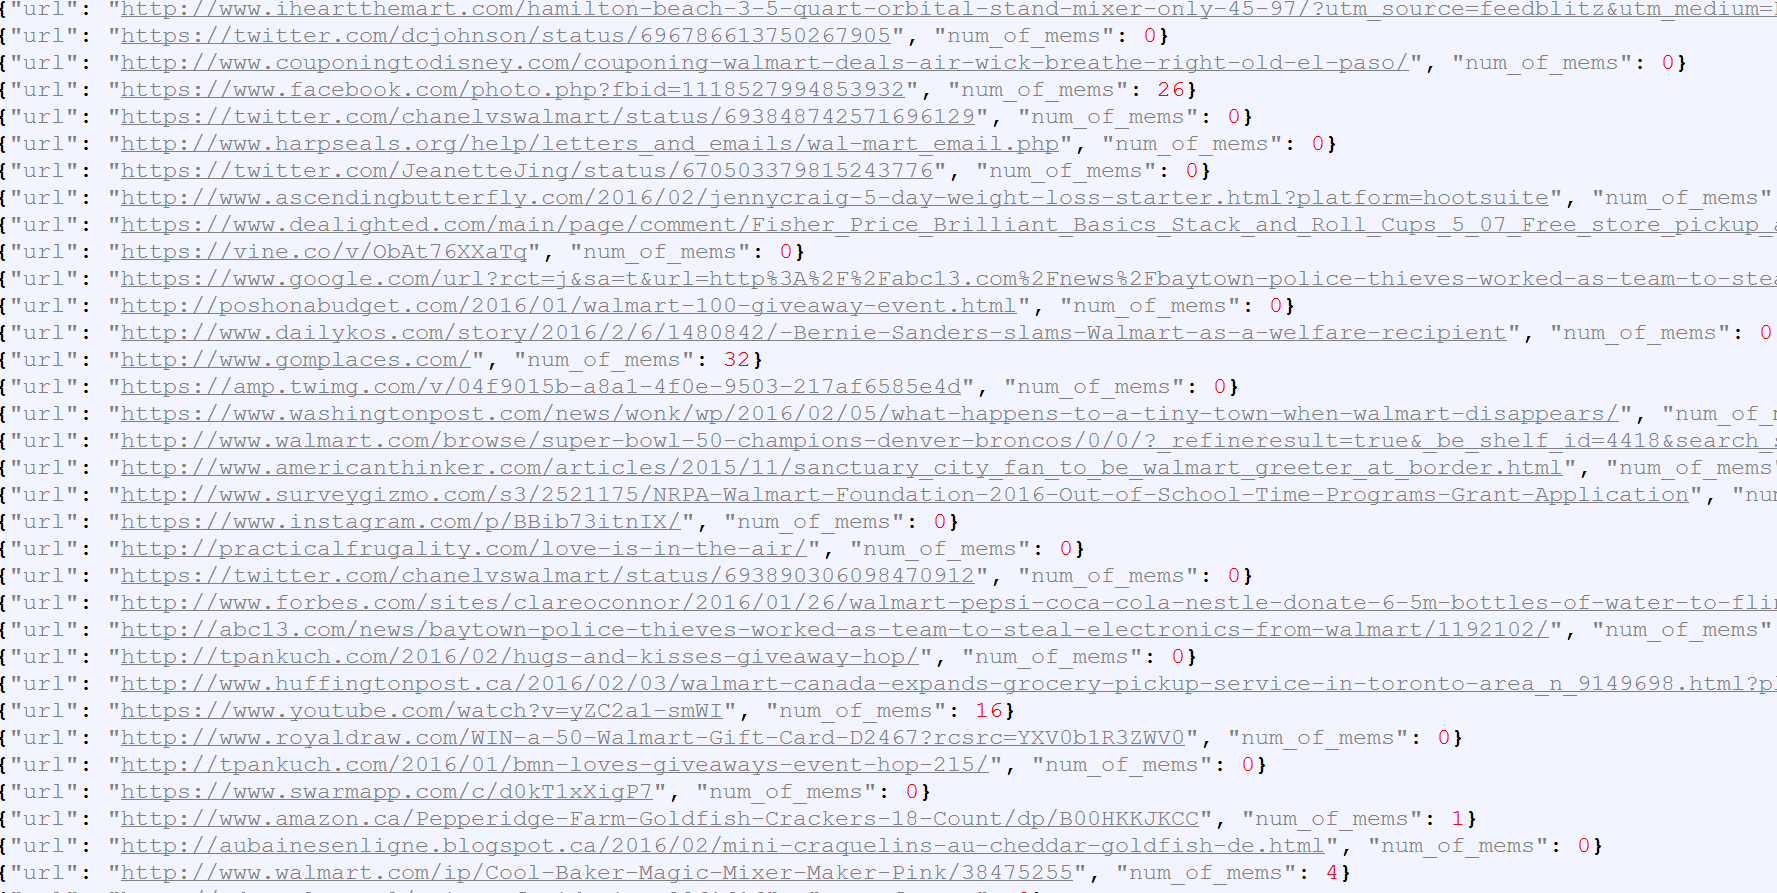
\includegraphics[scale=0.37]{output_mem_and_links.png}
        \caption{Links along with the number of mementos}
        \label{Links along with the number of mementos}
    \end{center}
\end{figure}
\newpage
\subsubsection{Urls with Mementos greater Zero}
\begin{figure}[ht]    
    \begin{center}
        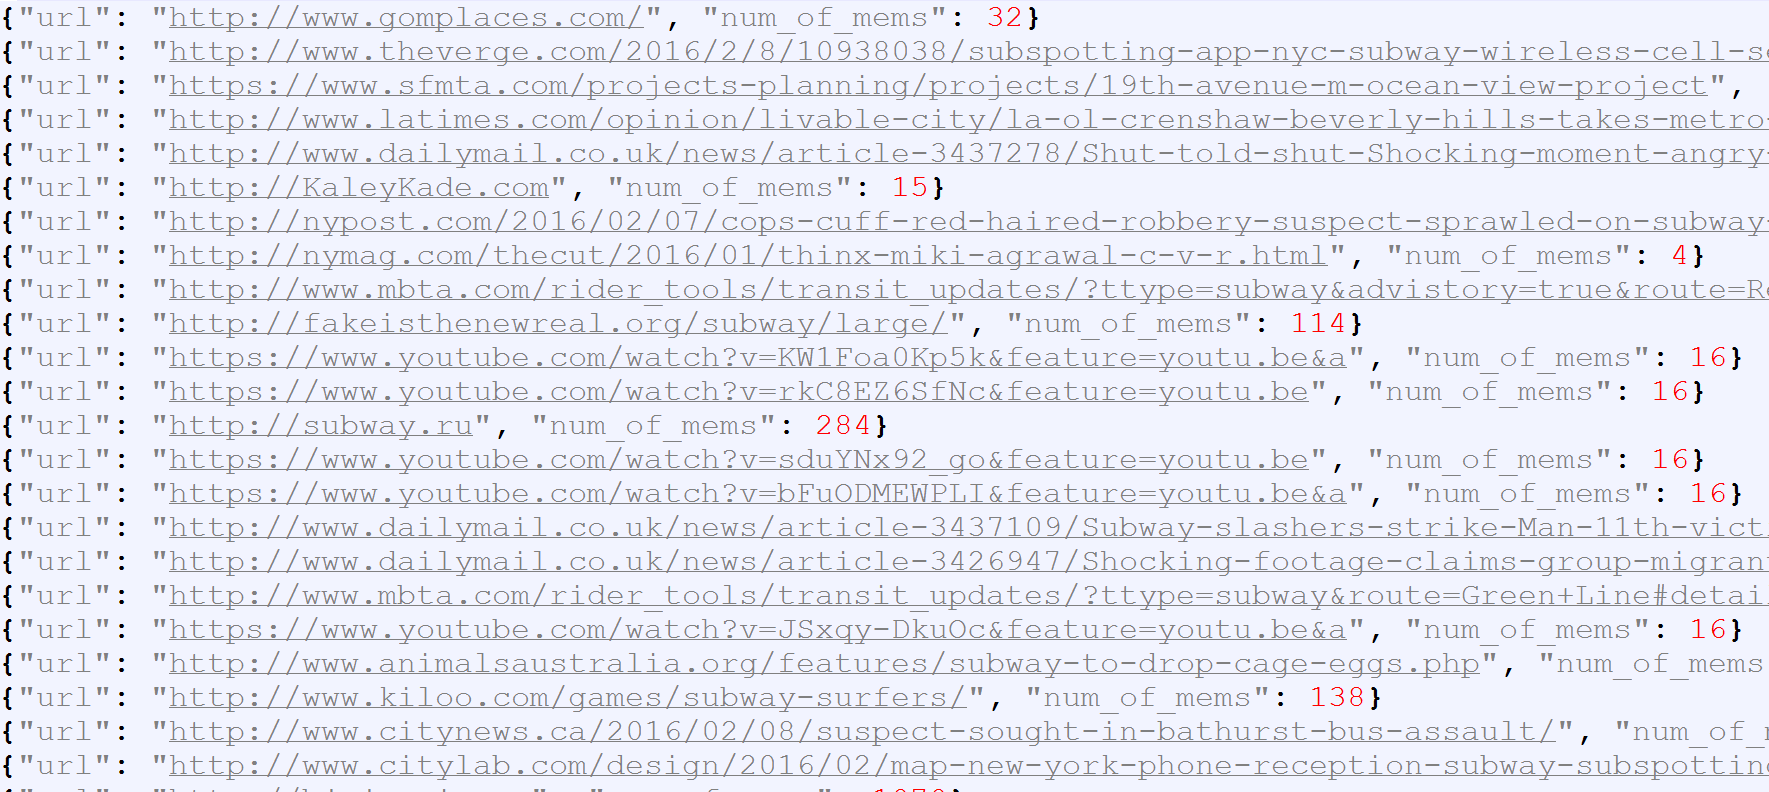
\includegraphics[scale=0.37]{mem_great_zero.png}
        \caption{Links along with the mementos greater than zero}
        \label{Links along with the mementos greater than zero}
    \end{center}
\end{figure}
\newpage
\subsubsection{Mementos count}
\begin{figure}[ht]    
    \begin{center}
        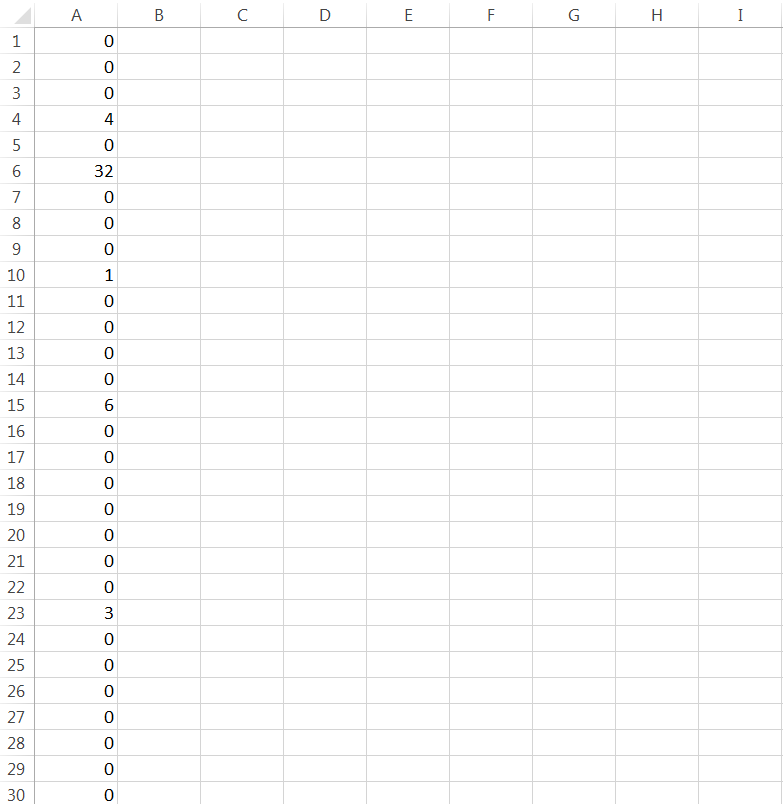
\includegraphics[scale=0.80]{allmems.png}
        \caption{Excel sheet with count of number of mementos}
        \label{Excel sheet with count of number of mementos}
    \end{center}
\end{figure}
\newpage
\subsubsection{Histograms}
\begin{figure}[ht]    
    \begin{center}
        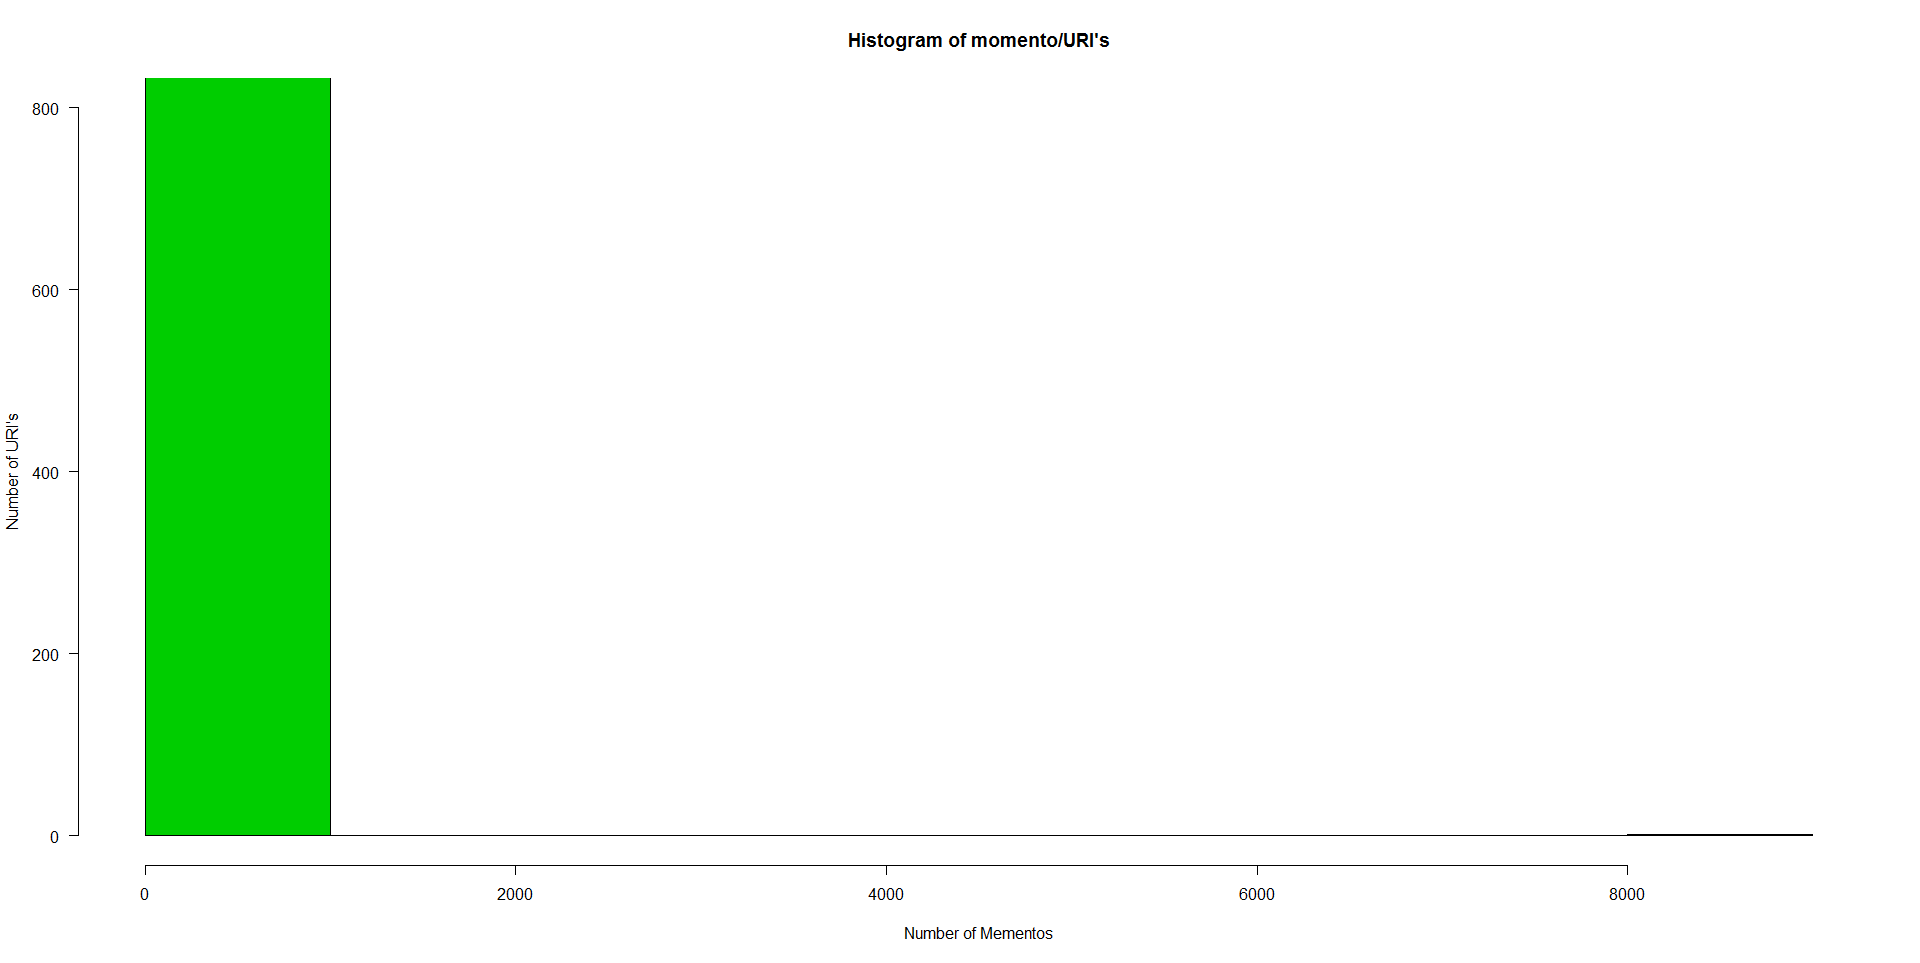
\includegraphics[scale=0.27]{histgora_bscale.png}
        \caption{Histogram 1}
        \label{Histogram 1}
    \end{center}
\end{figure}
\begin{figure}[ht]    
    \begin{center}
        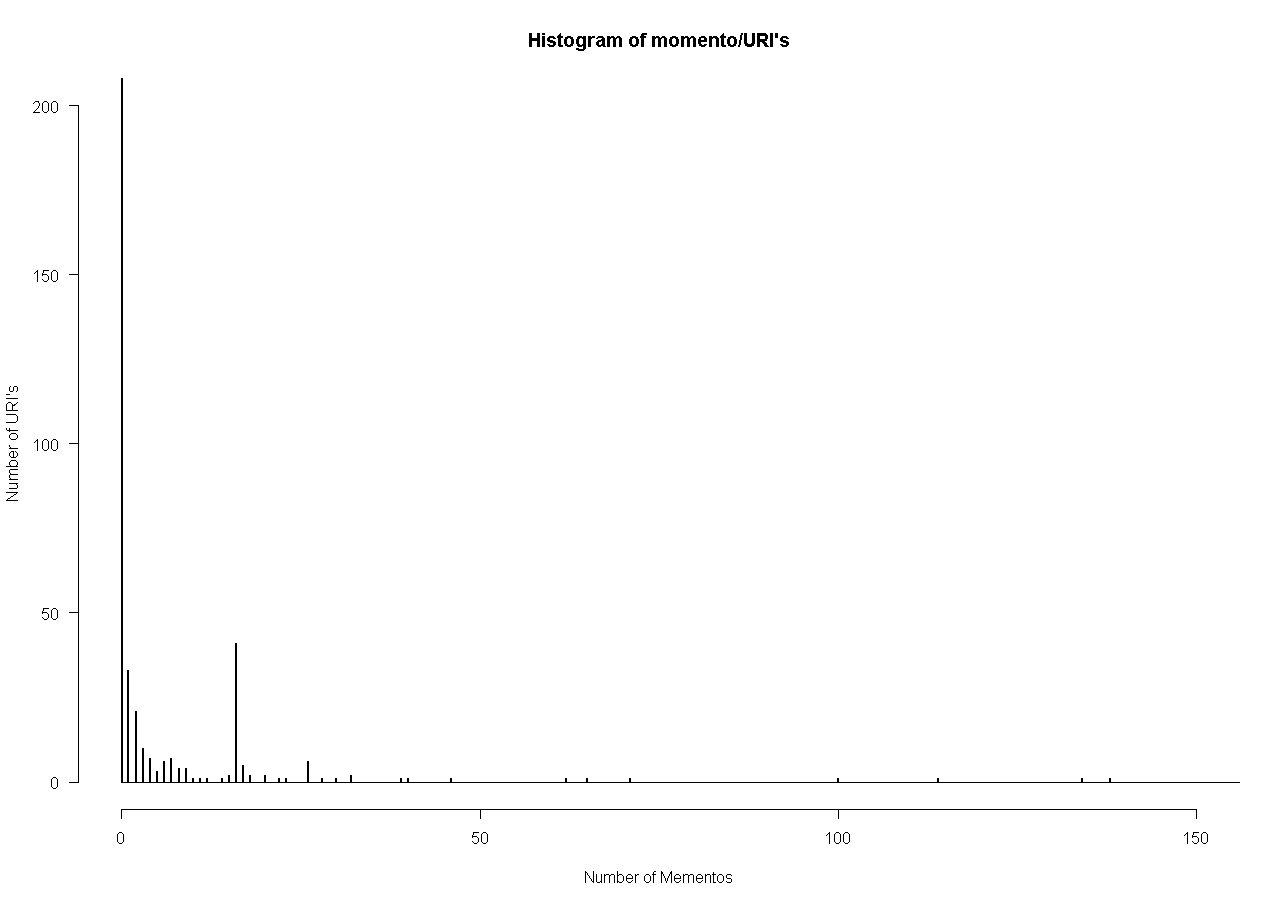
\includegraphics[scale=0.40]{histogram_mementos.png}
        \caption{Histogram 2}
        \label{Histogram 2}
    \end{center}
\end{figure}
\newpage
